\section{Control strategies}
Humans are capable of performing numerous dynamical movements in a wide variety of complex and novel environments while robustly rejecting a large spectrum of disturbances. Human movements such as a forward step and rapid arm rotations allow them to maintain overall balance in non-stability situations. Many researchers have studied how humans unwittingly use their body parts to recover balance as a response of external disturbances and make an approach for studying the stability of humanoid robots.

When the humanoid robot is in a stable posture, perturbantions may appear and they can be classified according the direction of action of that perturbations. All of them can be decomposed in anteroposterior disturbances (sagittal plane) and mediolateral disturbances (frontal plane). Studies of quiet stance have suggested separate postural strategies for balance in both planes depending on the stance position \cite{Winter1996}. There are three main mechanisms that can be applied to regain balance in such planes depending on the level of the disturbance: ankle, hip and step strategies.

The first is the ankle strategy. This strategy is applied in the sagittal plane or anteroposterior disturbances. For low intensity disturbances, the body can be considered as a nearly stiff pendulum, and balance adjustmensts are mainly made in the ankle joint, with the body balancing like a single inverted pendulum (Nashner, 1985). 

In the hip strategy, the resulting motion is mainly applied to the hip joints (Horak, et al. 1990). It can be applied independently or in combination of the ankle strategy. The hip joint movement is triggered when the external disturbance increases and the ankle strategy is not enough to keep balance. The hip strategy, same as ankle one, acts in the anteroposterior direction.

The last one is the step strategy. When these postural corrections become insufficient, the base of support must be adjusted (Carr, et al. 1987; Horak, et al. 1990). The modification of the support base leads new balance stability limits.

Figure (¿?) sumarizes this three strategies and Figure \ref{fig:strategies} shows the levels for strategy triggering. These limits are not fixed and they depend of the humanoid design as the sole surface or the height of the whole body, environmental conditions, i. e, standing in a flat surface has different strategy limits than in a narrow surface.

\begin{figure}[!htbp]
\centering
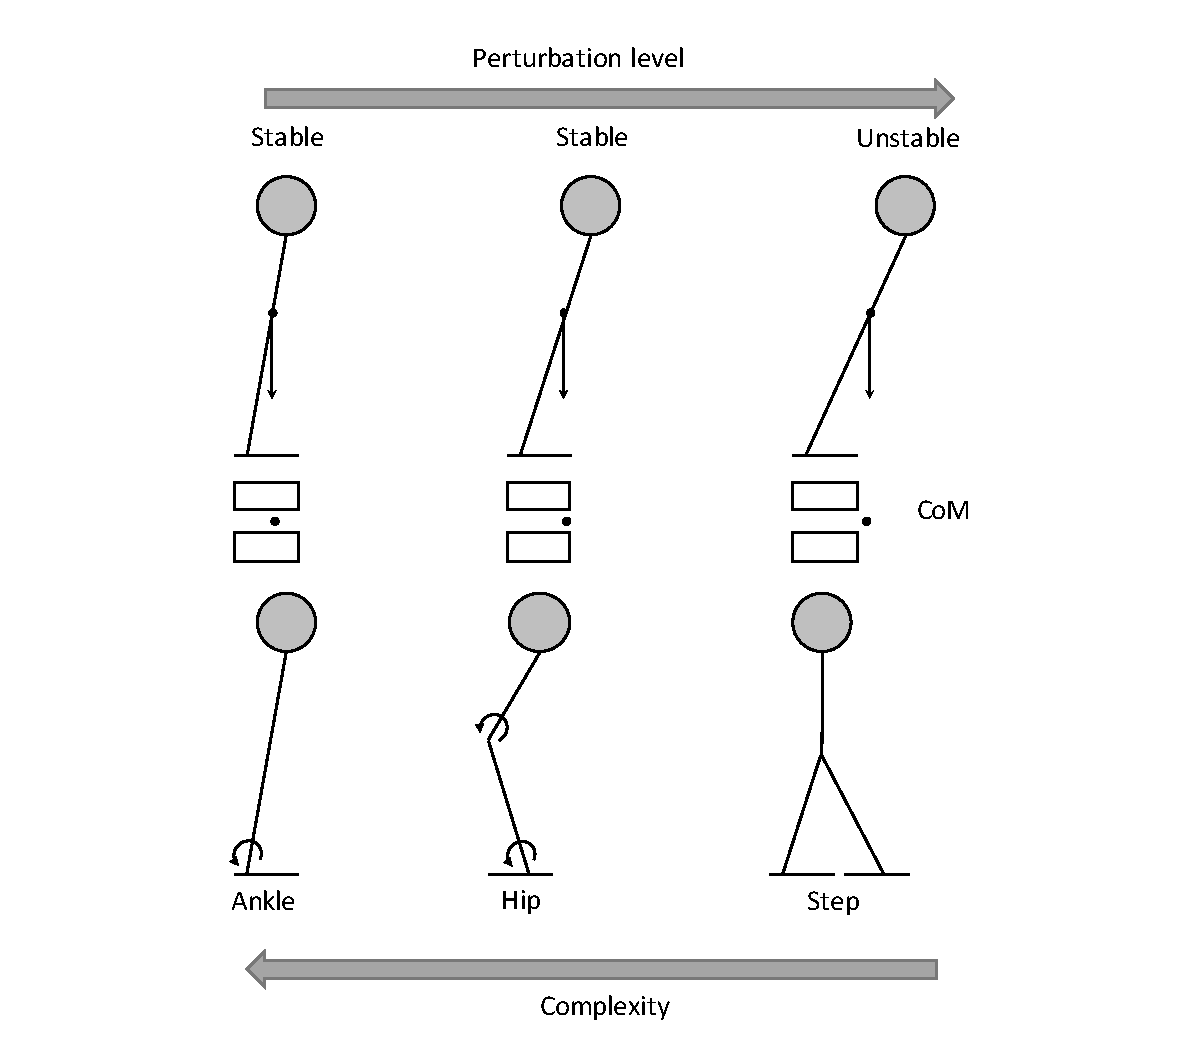
\includegraphics[scale=0.5]{strategies.pdf}
\caption{Recovery strategies.} \label{fig:strategies}
\end{figure}

In the mediolateral direction or frontal plane, the disturbances are compensated by the lateral movement of the hip joint in the case of upright stance. Double support in frontal plane, means there are two support points and a pendulum can not be considered. Both legs and the trunk of the robot make a parallelogram with the ground (see Figure \ref{fig:piernas} (a)). If a disturbance appears, and the hips maintain their perpendicular angles to the body, the feet will begin to loose contact with the ground as shown in Figure \ref{fig:piernas} (b). Then, to maintain stability, the angles of the parallelogram must keep on their relationship without loosing contact between feet and the ground, and the motion is applied to ankle and hip joints (Figure \ref{fig:piernas} (c)). 


\begin{figure}[!htbp]
\centering
\subfigure[]{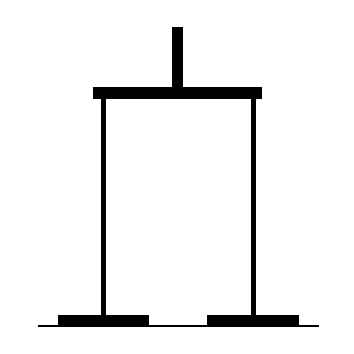
\includegraphics[width=40mm]{piernas1.pdf}}
\subfigure[]{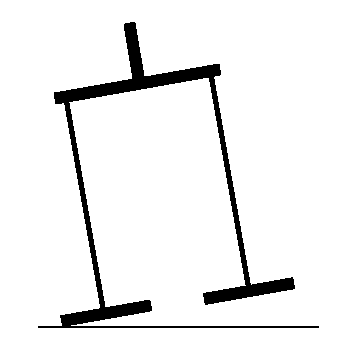
\includegraphics[width=40mm]{piernas2.pdf}}
\subfigure[]{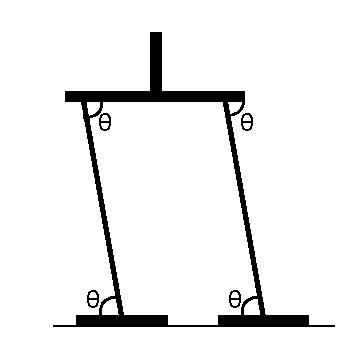
\includegraphics[width=40mm]{piernas3.pdf}}
\caption{Influence of hip and ankle angles in the frontal plane stability.} \label{fig:piernas}
\end{figure}

